\section{Stakeholder Analysis}

To properly plan the system, the stakeholders and their roles need to be identified. Figure \ref{fig:stakeholder-onion} shows a visual representation of stakeholders using a onion model.

\subsection{Onion Model}

\begin{figure}[H]
    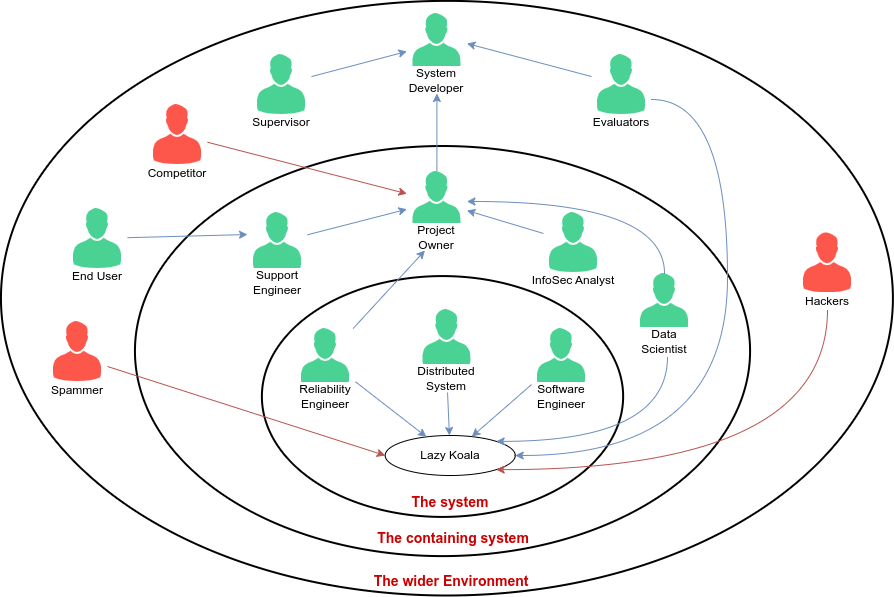
\includegraphics[width=15cm]{assets/requirement-specification/onion-model.png}
    \caption{Stakeholder onion model (self-composed)}
    \label{fig:stakeholder-onion}
\end{figure}


\begin{longtable}{|p{35mm}|p{44mm}|p{72mm}|}
    \hline
    \textbf{Stakeholder} &
    \textbf{Role} &
    \textbf{Viewpoint} 
    \\ \hline
    
    Reliability Engineer &
    Functional Beneficiary &
    Use the proposed system to understand issues quickly. \\ \hline
    
    Software Engineer &
    Functional Beneficiary &
    Use the proposed system to debug issues quickly. \\ \hline
    
    Distributed System &
    Functional Beneficiary &
    Become more reliable thanks to lower down time and \ac{mttr}. \\ \hline
    
    Project Owner &
    Financial Beneficiary &
    Owning a very useful tool that can be licensed to enterprise companies. \\ \hline
    
    System Developer &
    Financial Beneficiary &
    Sharpen the development skills and developer portfolio while earning royalty. \\ \hline
    
    Support Engineer &
    Functional Beneficiary &
    Less time dealing with frustrated users. \\ \hline
    
    End Users &
    Functional Beneficiary &
    Enjoy a more reliable product. \\ \hline
    
    Data Scientist &
    Functional Beneficiary &
    Expand upon the concepts and models created for the project. \\ \hline
    
    InfoSec Analyst &
    Functional Beneficiary &
    Use the anomaly detection algorithm to find unusual activities. \\ \hline
    
    Evaluator & 
    Advisory &
    Expand tools and technologies available in the field of reliability engineering. \\ \hline
    
    Supervisor &
    Advisory &
    Provide guidance to supervisee so they can successfully complete the project. \\ \hline
    
    Spammer &
    Negative stakeholder & Creates abnormal behaviors to trigger false alarms and waste developer time and resources. \\ \hline
    
    Hacker &
    Negative stakeholder &
    Exploit the proposed system and gain illegal access to the monitored system. \\ \hline
    
    Competitor &
    Negative stakeholder &
    Try to replicate results to expand their market share. \\ \hline
\caption{Stakeholder description (self-composed)}
\end{longtable}